\subsection{Gaussian Radial Basis Kernel}\label{Section1.3}

Although there are many kernels to use at our disposal, we turn our attention to a specific class of kernel that shall be used extensively in the upcoming theory and experimentation.

\begin{defe}[Gaussian Radial Basis Kernel] \label{defe: grbfk}
    For $d \in \NN, \; \sigma \in \RR_{>0}$ and $ \bm{z} , \bm{z}' \in \RR^d$ we define
    \[
        k_\sigma \left( \bm{z} , \bm{z}' \right) \triangleq \exp \left( - \sigma^{-2} \sum_{j=1}^{d} \left( {z}_j - {{z}'}_j \right)^2 \right).
    \]
    Then $k_\sigma$ is a real valued kernel called the Gaussian Radial Basis Kernel (RBF) kernel with bandwidth $\sigma$. Moreover $k_\sigma$ can be computed as
    \[
        \exp \left( \frac{- \norm{\bm{z} - {\bm{z}'}}_{2}^{2}}{\sigma^2} \right)
    \]
    \cite{SteinwartIngo2008SVMb}.
\end{defe}
The Gaussian RBF kernel makes for a very simple and intuitive measurement of similarity between its inputs. One geometric interpretation of the Gaussian RBF kernel is that as the radius of the smallest $d$-sphere containing $\bm{z} , \bm{z}' \in \RR^d$ grows the corresponding measurement of similarity decays exponentially. A visual representation of this decay is shown in Figure \ref{fig: grbfk_graph_1}.

\begin{figure}[H]
    \centering
    \subfloat{
        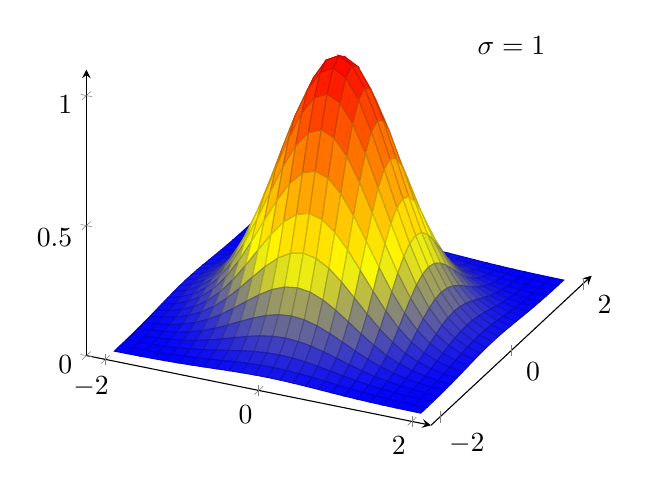
\begin{tikzpicture}

            \begin{axis}[
                    width=8cm,height=8cm,
                    domain=-2:2,
                    xmax=2.25,
                    ymax=2.25,
                    xmin=-2.25,
                    ymin=-2.25,
                    zmax=1.1,
                    axis lines = left,
                    colormap/hot,
                ]

                \addplot3[samples = 25, surf] {exp(-(x^2 + y^2)/1)};
                \node at (rel axis cs:1,0.5,1) [above] {\(\sigma=1\)};

            \end{axis}

        \end{tikzpicture}
    }%
    \quad
    \subfloat{
        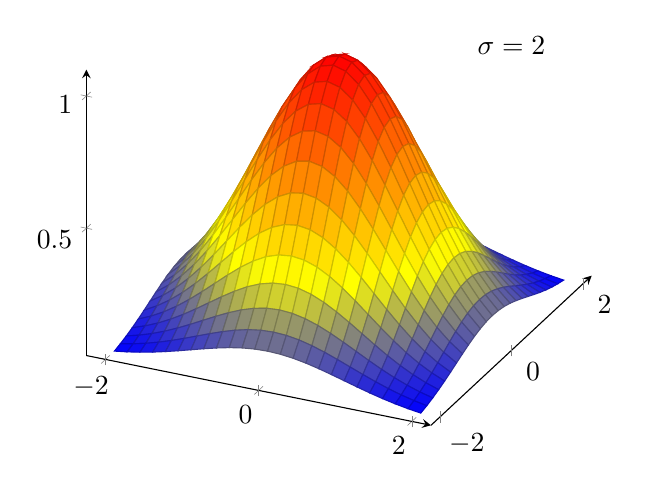
\begin{tikzpicture}

            \begin{axis}[
                    width=8cm,height=8cm,
                    domain=-2:2,
                    xmax=2.25,
                    ymax=2.25,
                    xmin=-2.25,
                    ymin=-2.25,
                    zmax=1.1,
                    axis lines = left,
                    colormap/hot,
                ]

                \addplot3[samples = 25, surf] {exp(-(x^2 + y^2)/2)};
                \node at (rel axis cs:1,0.5,1) [above] {\(\sigma=2\)};

            \end{axis}

        \end{tikzpicture}
    }%
    \caption{A graph of the Gaussian RBF from definition \ref{defe: grbfk} for $d=2$. Evidently, a larger value of $\sigma$ slows the rate of decay increasing the similarity between the same pair of samples.}%
    \label{fig: grbfk_graph_1}
\end{figure}

This kernel is infinitely differentiable meaning it has mean square derivatives of all orders and is therefore very smooth. In fact, some argue that such strong smoothness makes it unrealistic for modelling natural phenomena \cite{RasmussenCarlEdward2006Gpfm,SteinMichaelL1999IoSD}. Nontheless, Gaussian RBF kernels remain the one of the most widely used in literature.